% 图 23.1 —— 由 `checks/emit_hand.py` 自动拼出（probe 精测 + prims2 图元分解）
%%
% ⚠ 这是**稿子不是成品**：跑 `checks/checkhand.py 23.1` 看指标 + 看叠合图。
%%
%% ⚠ 待核：
%   · 本图 probe 报出阴影族 1 个 —— **本脚本不生成阴影**（要照原书手写）；prims2 的 strokes 里可能含阴影线，核对时留意别画重
%   · 可疑字形 1 项（空心圈 ⊙ 常被认成字母 o）—— 见文件末
%%
\documentclass[12pt]{standalone}
\usepackage{fontspec}
\setsansfont{Arial}
\newfontfamily\mfallback{DejaVu Sans}
\usepackage{tikz}
\begin{document}
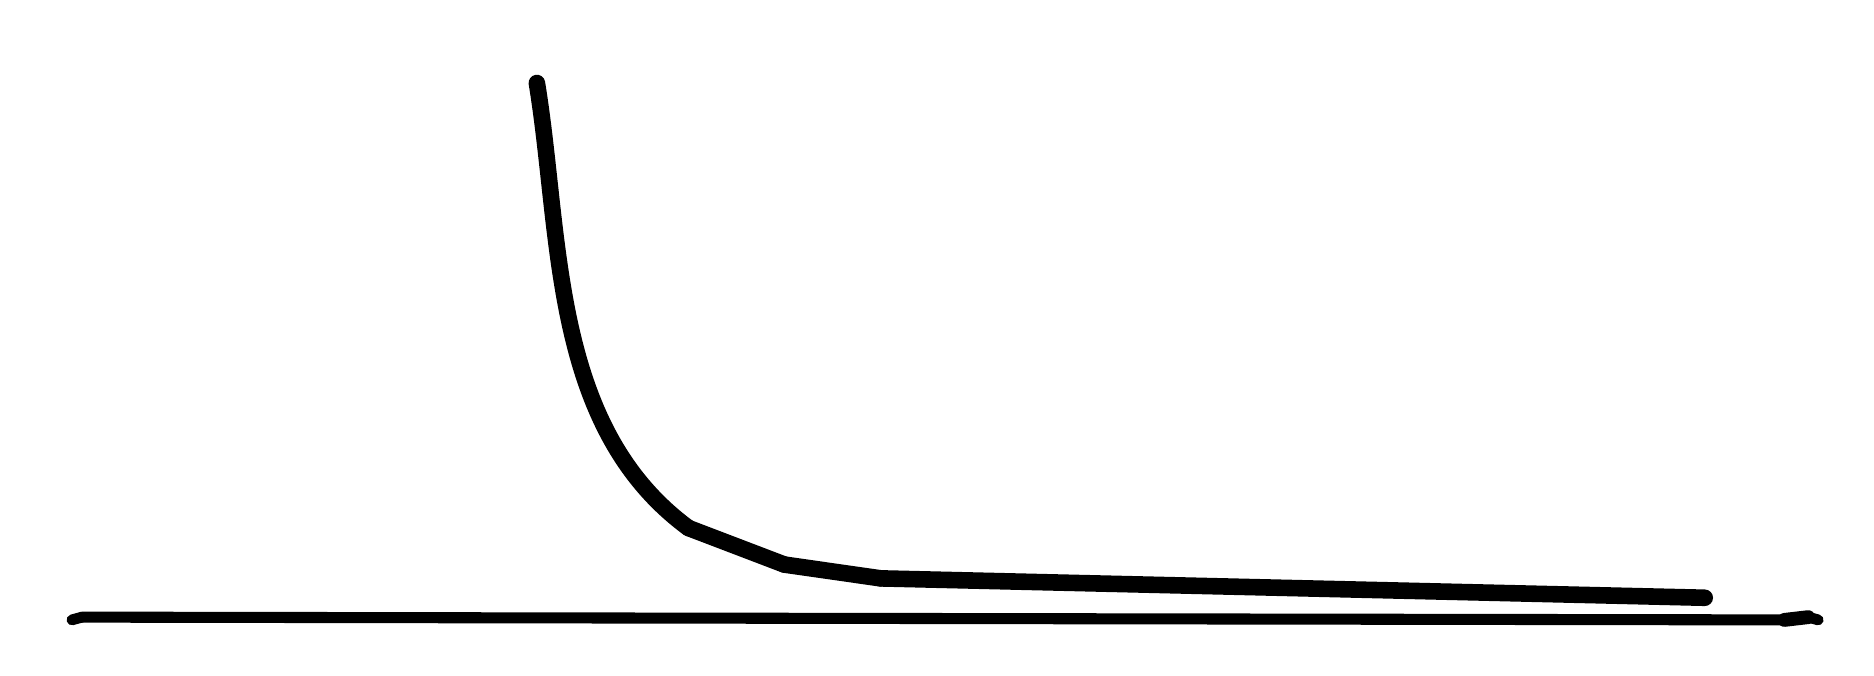
\begin{tikzpicture}[x=1pt, y=-1pt, line width=3.9pt, line cap=round, line join=round]

  %% ════ 直线段（prims2 的 strokes）════
  \draw[line width=3.9pt] (16.0,214.0) -- (19.6,213.0);
  \draw[line width=4.0pt] (19.6,213.0) -- (634.8,214.0);
  \draw[line width=5.0pt] (634.8,214.0) -- (643.4,213.0);
  \draw[line width=3.9pt] (643.4,213.0) -- (647.0,214.0);
  \draw[line width=6.0pt] (606.0,206.0) -- (308.3,199.0);
  \draw[line width=6.0pt] (308.3,199.0) -- (273.4,194.0);
  \draw[line width=6.0pt] (273.4,194.0) -- (238.8,180.8);

  %% ════ 曲线（prims2 的 curves —— 三段式，坐标同为 (y,x)）════
  \draw[line width=6.0pt] (238.8,180.8) .. controls (188.7,143.9) and (193.1,75.8) .. (184.0,20.0);

  %% ════ 标签（probe 直接给的 \node 行）════
  %% ⚠ 全部补了 fill=white：文字在最上层，否则与曲线交叉干扰

  % 钉死画布：否则超出的图元/控制点会把页面撑大，1:1 回比就失准
  \pgfresetboundingbox
  \path[use as bounding box] (0,0) rectangle (657,224);
\end{tikzpicture}
\end{document}

% ⚠ 待核清单（probe 拿不准，人眼过一遍）：
%   · 未识别/跳过：⑤ 跳过/未识别的字形
